%---------------------------------------------------------------------------------------------------
% Analysis
%---------------------------------------------------------------------------------------------------
\newpage
%\part{Anfang}
\chapter{Analysis}\label{cap:Analysis}
In the beginning, it is major important to analyze the target group, the necessary surrounding for developing an Android application, and of course, the existing Civitas project. Furthermore, it makes sense to consider what outcome is desirable.

\section{Target Group}
Since this Civitas project was started at the University of Hamburg from the historical faculty, it was designed as an educational tool to collect information about historical monuments. In this context, a historical monument became known as a so-called artefact. Therefore, its task is to provide a frame for visual, textual, and audio information. These artefacts should be created, maintained, collected and discussed by its target group, the students of history studies and historically interested people. It is assumable that the target group remains manageable. A growth development, for example, like Facebook or Twitter, has experienced, is not expected. 
% We keep this aspect in mind and return on it during the analysis part of this thesis. 


\section{Tools}
The most applications were created within so-called Integrated Development Environments (IDE). The Civitas app makes no exception, so it was built with Android Studio (\textbf{AS}). \textbf{AS} is the primary tool for developing Android applications. It supports Java and Kotlin as native programming languages. As the app was written in Java, it will continue to be developed in Java.
Here is a brief overview of the used tools during this bachelor thesis.

\subsection{Android Studio}
\textbf{AS} is the official IDE for Google's Android operating system. 
There are many features, like code templates, auto-suggestion, and operation shortcuts, to name a few of them, that will make app development enjoyable. A complete list would be out of the scope of this bachelor thesis, so it will not be discussed further. The result from an \textbf{AS} project is called an app. An app consists mainly of two parts: 1. \textbf{Java}-based code files, and 2. layout files based on \textbf{XML}.  

\subsection{Java}
Java is an object-oriented programming language. Compiling Java source code results in a binary program-code, the bytecode. This bytecode runs through the runtime-interpreter of the Java Virtual Machine (JVM) and becomes translated into the machine code of the hosting operating system. Therefore, Java gets one of its central properties, operating system independence. It has a large community, so that problems can be discussed quickly and the chance of helpful answers is quite significant. Long story short, within \textbf{AS} projects Java is responsible for the app logic.

\subsection{XML}
XML stands for e\textbf{X}tensible \textbf{M}arkup \textbf{L}anguage. It \textit{"defines a set of rules for encoding documents in a format that is both human-readable and machine-readable"} \cite{wiki:xml} and is used for representing data. Within an AS project, XML will define the graphical layout of the application.

\subsection{Git}
Today's software development is strongly tied to Version Control Systems (VCS). Complex projects, parallel working within a team, proper documentation, distribution of tasks, and code reviews are some of the main benefits of VCS. There are numerous different VCS providers available, like GitLab, GitHub, and others, but they all work quite similar. One has a local project folder, called repository, and another online remote repository. Saving changes to the local project is called commit. This commit comes along with related information about the change (commit message). Hence, it is easy to follow the development process. The push command applies the local commits to the remote repository. If the push is successful, the remote repository is up to date, and another software developer can fetch and pull the repository and continue developing with the latest version. 
This Civitas project is integrated into a GitHub repository and contains about 350 commits at the time when this document was written.
The link to the repository is stated within the appendix section.



\section{Current Civitas App}
% REST architecture
Since there were at least two iterations of starting/improving the Civitas app within a bachelor thesis background, it is worth to scope out the latest achievements.

The previous developer achieves, that the Civitas project \textit{"now has an Android application with a comfortable one-click login feature. The users of the application have an interface to exchange the image and audio information as well. The users and the administrators of the Civitas system also can edit and delete artefacts from the Civitas database."} \citep[p. 54]{Ganapijev18} 


Unfortunately, the Civitas project was not executable at the start of this thesis. This might be caused by crossplay of the following reasons:

\begin{itemize}
\item Google Sign-In
\item Server was paid from the previous developer
\end{itemize}

The Google Sign-In feature was implemented to manage the user registration and user login. To use the Google Sign-In, it is mandatory to configure a Google API Console project and setup your Android Studio project. 
In addition to the fact that the "server is being paid from the [previous] developer's budget" \citep[p. 51]{Ganapijev18}, which has been terminated after finishing his thesis, every server request attempt must fail. As a result, there were no server sided data available. 
Unfortunately, there was no instruction sheet within the appendix section of the previous developers' thesis neither for the Google Sign-In settings nor for the server structure. So it turns out that this is like looking for a needle in a haystack.

The resulting dilemma from this scenario leads to the problem the previous developer was also faced too. 
Spending a vast amount of time to figure out how the server software works or replacing the existing Back-end solution by a new approach using Back-end as a Service (BaaS).

The app experience of the current developer with the existing Civitas app relies on rarely 30 minutes of usage. This is caused by the problems stated above. Of course, the source code is available and has been appropriately analysed.

Consider the previous developers' advice, \textit{"that the Back-end must migrate at least once again."} \cite[p. 51]{Ganapijev18}

The decision was made to start with the \textbf{BaaS} approach, offered by \textbf{Backendless} with a free billing plan. 
The choice was affected by some facts worth to mention.
Backendless does not only provides a back-end for free, but it also delivers a web-application, user services, files storage system, geolocation section, and much more functionalities. Another argument pro Backendless is its easy usage, and that the future result is only depending on the Android Studio project, there is no need to care about the REST server application anymore.

The contra arguments were that the Backendless free billing plan does not support unlimited data resources.
Due to the previous assumption that the target group remains manageable, Backendless with its BaaS comes into play. The free billing plan provides a lot of features that fit the demands of an application that is within its test environment. If the project owner lifts its thumb, as Roman emperors did in the past, there is an easy and affordable upgrade possible, to improve the capacity of the Backendless storage amount.

So the next decision to take was to integrate the Backendless BaaS into the existing project or to start a whole new Civitas project. 
On the one hand, a lot of work was invested in the project; on the other hand, the predecessor needed a lot of time to get involved. Since the current developer has gained experience with Backendless, the web app is included and the back-end does not need to be developed, the focus is exclusively on the Android app. The resulting time savings allow to restart the Civitas project from scratch.
This decision was made on the premise of following the layout concept and generally adopting the useful aspects of the old version. Hence, it will be much easier for potential successors to develop the project further as the app is now much easier to put into operation.


\section{Desired Result}

A rebuilt should contain all functions of the existing Civitas project. 
Due to the predecessors future work advice, it would be appreciated to introduce a list of artefacts owned by the user for easier access. Furthermore, a search field and an admin control panel would be welcomed as well \cite[cf. p. 55]{Ganapijev18}.

In the end, it should contain an Android app, and a server sided back-end and an admin control panel.
To accomplish these desirables, it is useful to investigate the following aspects.

\subsection{Android App}
The Front-end is the visible part of the Android app presented to the user. It is responsible for the interaction between user and app and delegates events like button clicks to the underlying software logic. In this case of rebuilding the app, it should fulfil the same known requirements like the predecessor once stated, plus the additional features mentioned above. Here is the complete list:

\begin{itemize}
\item The user should be able to create an account and login into Civitas system
\item The users must be able to upload pictures and additional information
\item \sout{The application must support three different user account levels: regular users, trusted users and administrators}
\item The content uploaded by users must be automatically shown in the application
\item The app must include an interactive map, that shows the current location of the user as well as various artefacts on the map, that has already been added to the application
\item If the user clicks on a map marker, a pop-up window must appear showing the user additional information about the artefact
\item The app must include an artefact list overview
\item The app must be connected to an admin control panel
\item The stored artefacts must be sortable by various filter methods
\item The filtered results must be visible within the artefact list overview and/or the map
\item The user should be able to reset login credentials
\item The usability should be increased
\end{itemize}

Since the existing features were introduced within the previous study, now the focus lays on the newly added. Here is a brief introduction. 

\subsubsection{Artefact List Overview}

A lot of popular apps, like Netflix, eBay Kleinanzeigen, Chefkoch, etc. provide listed items to the user. A common way to display items in a list that contains images, as well as textual content is covered by using the recyclerview framework. The following image gives a brief overview of how popular apps provide content.

\begin{figure}[H]
	\centering 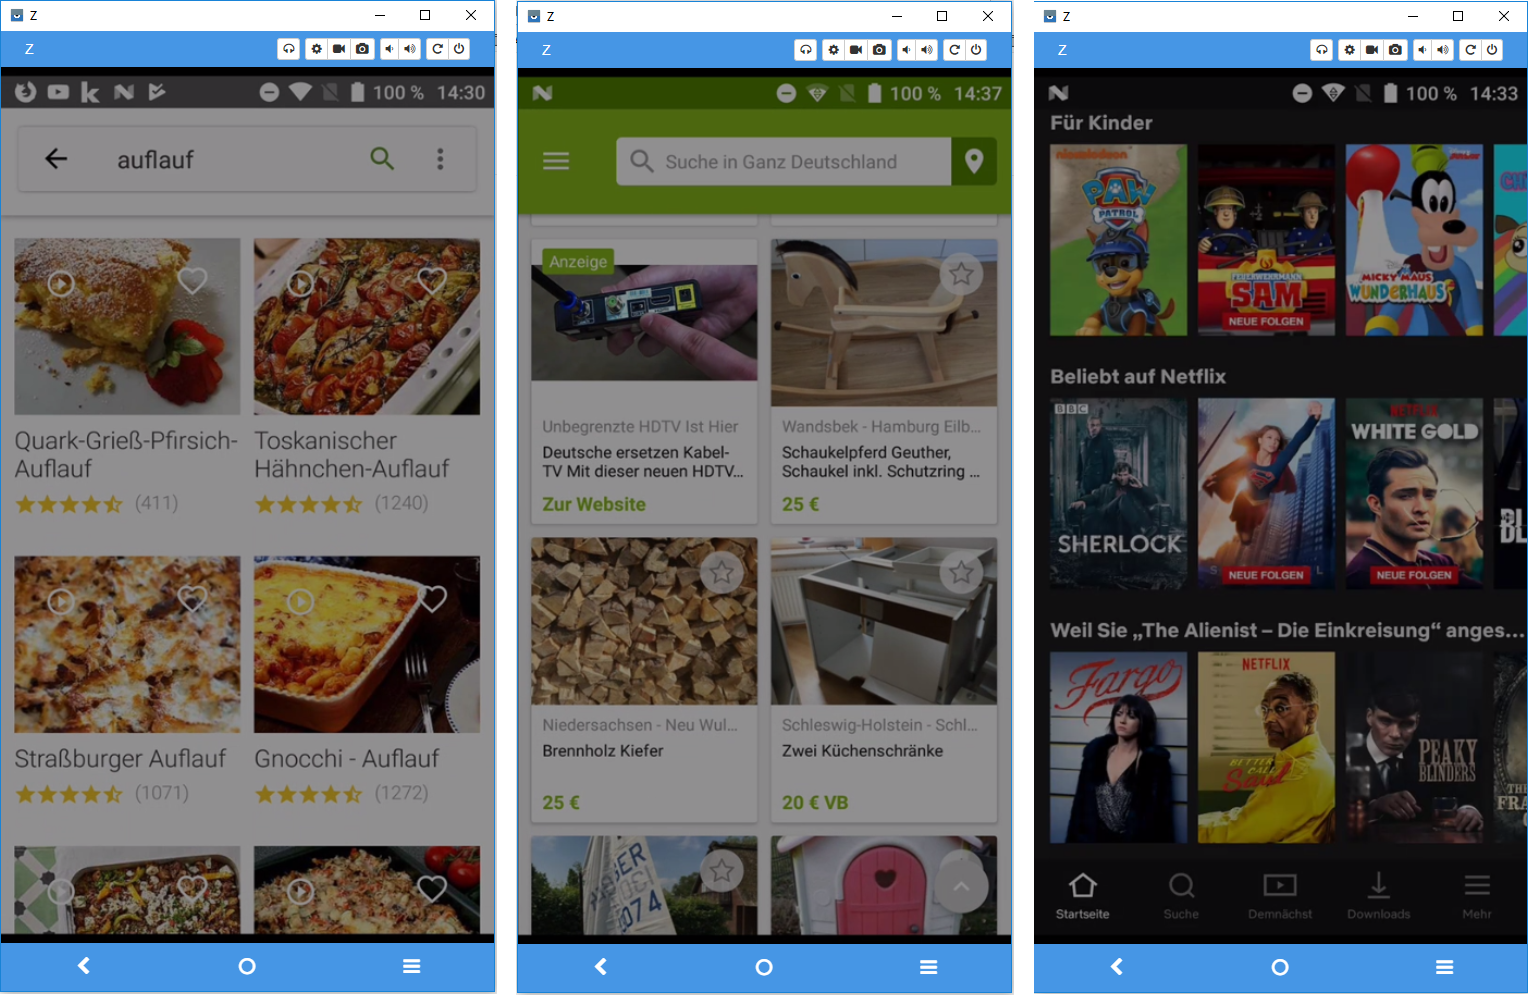
\includegraphics[width=0.8\textwidth]{recyclerview_overview.png}
	\caption[Popular apps with list overview]{Popular apps with list overview}
	\label{fig:recyclerview_overview}
\end{figure}

The single artefact items within this list overview should display specific artefact properties. There could be any information presented to the user, but for now, an item contains values for image, name, and category. 



\subsubsection{Filter}
The existing filter function in the Civitas app allows the user to choose a) filter by category and b) filter by date with a fixed limit.
Since nearly everybody is familiar with filter functions from everyday life, this way of filtering is quite ancient and depress the user experience. Therefor this part of the app should get a rework.
Ideally, the filter allows a single or combined search for a variety of parameters and displays the result as well on the google map represented by a marker, or within an artefact list overview. It would also be pleasant if the date is flexible so the user can search from any age to any other age. Additional another filter option for search by artefact author would be useful. This case would kill two birds with one stone because it is an elegant way to fulfil the predecessors' demands a list of artefacts owned by the user.

\subsubsection{Usability}
Increasing usability can mean everything and nothing. Here are some usability cases to provide an understanding. Using AsyncTasks to perform operations in the background, so the app is responsive to user inputs. Integrating progress indicators to the user interface. Centering the screen position smartly.



\subsection{Back-end}
The previous app was built with the REST architecture style. However, the new app follows a different approach, called \textbf{BaaS}. First of all, what is Baas? BaaS, also known as mBaaS, is an acronym for \textbf{m}obile \textbf{B}ack-end \textbf{a}s \textbf{a} \textbf{S}ervice. Deeper investigating into the question leads to these results.
"Platforms that perform the role of BaaS are prepared cloud server infrastructures that offer their backend job for most types of applications." \cite{4mbaasCompare}
They also offer features like registration and login services, standard data requests, push notifications, file storage, analytics, geolocation, integration in multiple operating systems, hosting, and many more. Long story short, with the words of \textit{George Batschinski} (Back4App founder), it "allows mobile/front-end developers to NOT have to develop the back-end." \cite{baasCompare}
A general pro and contra comparison using BaaS is in the following table (\ref{tab:baasProCon}).

\begin{table}[h]
\centering
\begin{tabular}{|l|l|}
\hline
\multicolumn{2}{|c|}{\textbf{BaaS}}     \\ \hline
\textbf{Pro}      & \textbf{Contra}     \\ \hline
save time         & no complete control \\ \hline
save money        & latency issues      \\ \hline
richer apps       & costs               \\ \hline
more productivity & vendor lock         \\ \hline
security          & -		            \\ \hline
\end{tabular}
\label{tab:baasProCon}
\caption{Pro and contra BaaS}
\end{table}

Of course, when one does not has to develop the back-end, it saves time, and therefore, money. One also can raise productivity and provide more vibrant apps, because one can focus on the essential parts of the app and offer features that one is maybe unable to implement. On the flipside of things, one is dependent on the company, and with increased utilization, one can deal with latency issues and costs. In 2016 the BaaS provider \textit{Parse} shut down the service and faced the customers with a vendor lock, which ends up in extra trouble and expenses for the customer.  

Now, with an idea of BaaS, it is worth to analyse the market situation and the providers. Consulting the internet results again with an entry of \textsc{George Batschinski}.\textit{ "Backend as a Service market is growing very fast, and it will reach US\$ 30 Billion in 2019... So, the BaaS becomes one of the hottest markets in tech and will support the fastest growing professional segment in the world."} \cite{baasProCon}
Various BaaS companies were competing for market shares. One has to consider the functionalities of the Civitas app to select the most fitting provider. Apigee, StackMob, Kumulos, App42, Back4App, Backendless, to name a few of them. A detailed comparison is not the subject of this thesis, so it will not be discussed further.
In addition to the fact that the current developer has already gained experience with Backendless, the decision to choose BaaS from Backendless was made for the following reasons. It comes along with a convenient and easily understandable web application, has an excellent file storage system, supports geolocations with metadata information, offers proper user management, easy API request pattern, and extensive documentation. It also has a suitable pricing policy, including a free billing plan, which is sufficient for the early phase of the Civitas app. One can upgrade the limits by changing the billing plan, and/or ordering an additional function pack for the desired property, at later stages. A detailed price-performance ratio is displayed in the following image (see \ref{fig:pricing_plan}). 

\begin{figure}[H]
	\centering 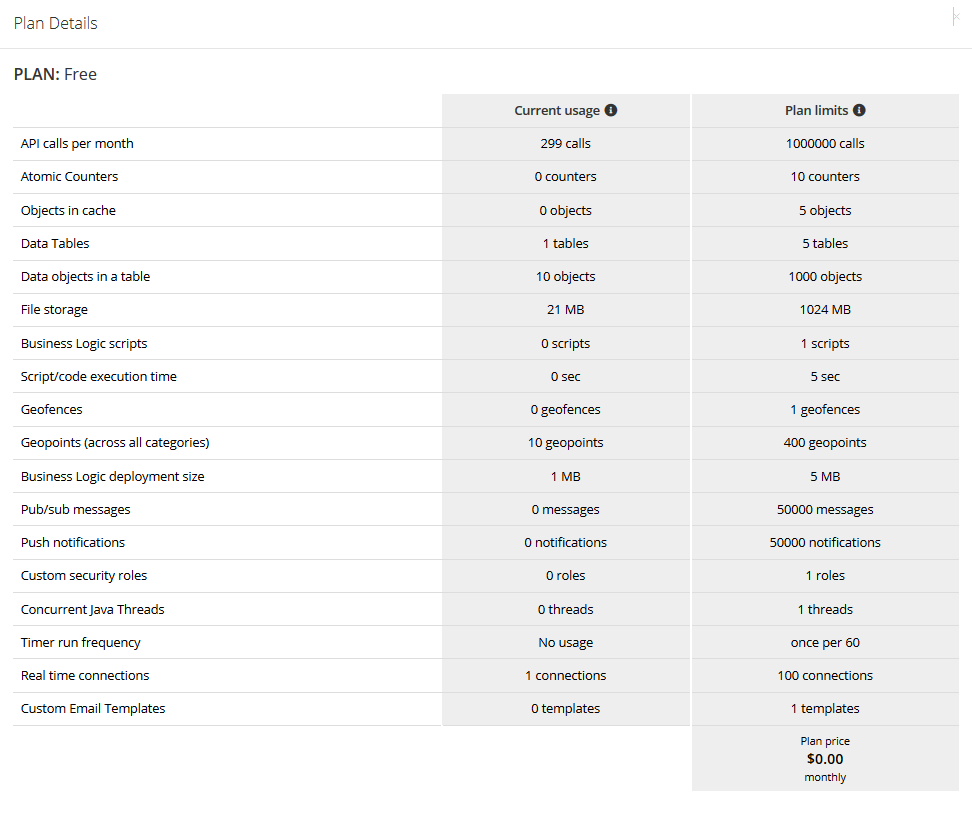
\includegraphics[width=0.8\textwidth]{analysis/pricing_plan1.png}
	\caption{Backendless pricing plan}
	\label{fig:pricing_plan}
\end{figure}

One can calm customers' minds, fearing a vendor lock, Backendless Founder Mark Piller says, \textit{"your data belongs to you... We hope you never want to leave, but if you do, exporting out everything is part of the Backendless management console. You can reconstruct the entire app anywhere, anytime."} \cite{badassBackendless}

To summarize this section, as a result of using BaaS instead of the formerly used REST architecture, the Civitas project gains an Android app, a back-end solution and a web app that acts as an admin control panel. Hence, the demands of this iteration process are fulfilled, and one can continue with the implementation of these, within the next chapter.








